\documentclass[10pt,twocolumn]{article}

% use the oxycomps style file
\usepackage{oxycomps}

% usage: \fixme[comments describing issue]{text to be fixed}
% define \fixme as not doing anything special
\newcommand{\fixme}[2][]{#2}
% overwrite it so it shows up as red
\renewcommand{\fixme}[2][]{\textcolor{red}{#2}}
% overwrite it again so related text shows as footnotes
%\renewcommand{\fixme}[2][]{\textcolor{red}{#2\footnote{#1}}}

% read references.bib for the bibtex data
\bibliography{references.bib}

% include metadata in the generated pdf file
\pdfinfo{
    /Title (Senior Comps Proposal: Generating and Evaluating Synthetic Macroeconomic Time Series)
    /Author (Kincaid Fries)
}

% set the title and author information
\title{Senior Comps Proposal: Generating and Evaluating Synthetic Macroeconomic Time Series}
\author{Kincaid Fries}
\affiliation{Occidental College}
\email{kfries@oxy.edu}

\begin{document}

\maketitle

\section{Introduction}

\subsection{Background}
The use of machine learning in financial prediction has grown rapidly due to its ability to model complex, multivariable relationships and generate realistic predictions. Machine learning is particularly effective in equities markets where thousands of points of training data are available daily for stock movements. In contrast, macroeconomic data takes months of study, surveying, and research to come up with even a single realistic measurement. Consequently, macroeconomic forecasting models rely on quarterly historical data at best. \textcite{baltazar2020sustainableeconomies} note that small datasets affect the reliability of macroeconomic modelling. Other challenges like changes in calculation methods, unavailability of data for certain time periods, and changes in indicator definitions make it hard to train macroeconomic models without overfitting to small datasets. Recent advances in synthetic data generation offer a promising alternative, allowing researchers to create realistic simulations of economic behavior without relying solely on historical data.

\subsection{Goal}
The goal of my senior comprehensive project is to evaluate whether a machine learning model trained on macroeconomic datasets can be used to generate realistic synthetic data. By normalizing macroeconomic indicators across different economies, I hope to address the issue of relatively limited time-series for a single country by taking training data from multiple countries. My project will explore whether synthetic time-series produced by a model trained on data from multiple countries can serve as a valid counterpart to real economic data in forecasting applications.

The model will be trained to learn the underlying dynamics and structure of macroeconomic movements in developed, free-market economies. To evaluate whether the generated synthetic data is realistic, I will first compare statistical properties of the synthetic data with real world data. Particularly, I will be focusing on the distribution of the data, to determine whether the movements in the synthetic dataset are similar to the movements of real data. Additionally, I will compare the performance of two forecasting models, one trained on real data and the other on synthetic data, in order to predict future GDP movements or other economic indicators. I will compare how these two models perform in terms of making accurate predictions about real macroeconomic data on a held-out real dataset. If the forecasting model trained on synthetic data performs similarly to the model trained on real data, then that would suggest that my method of synthetic data generation is viable for emulating real economic patterns. By looking at both statistical factors and comparing forecasting model performance, I hope to thoroughly assess the viability of the synthetic data.

\section{Technical Background}

\subsection{Macroeconomic Indicators}

\subsubsection{Overview}
Macroeconomic indicators refer to data points which are revealing of the state of the entire economy. They are impactful to all levels of finance and the economy, and are even politically salient, as \textcite{ravallion2021macroeconomicmisery} notes the impact of macroeconomic indicators on electoral outcomes. The macroeconomic indicators that I will focus on will be consumer price index (CPI), unemployment rate (UR), real wages (RW), and gross domestic product growth (GDP), which were selected based off of the research of  \textcite{ravallion2021macroeconomicmisery} and \textcite{baltazar2020sustainableeconomies}.

\subsubsection{Selected Indicators}
\begin{itemize}
  \item \textbf{CPI}: measures of the price of a pre-defined theoretical ‘basket’ of goods; where changes in CPI over time are used to calculate the inflation rate. The ‘basket’ is a collection of common household goods which every individual regardless of income level will regularly purchase.  
\item \textbf{UR}: is the proportion of the labor force actively seeking work to the total number of people in the labor market. A very low unemployment rate places upward pressure on salaries due to the high competition in the workforce. A high unemployment rate means there are a significant number of individuals without income seeking employment. The efficient unemployment rate is typically around 5\% \cite{voxeuUnemployment}.
  \item \textbf{RW}: reflects the inflation-adjusted earnings of the average worker, capturing not just the gross amount of money an individual in the economy is expected to bring in, but also the purchasing power that amount of money affords \cite{treasuryRealWages}.
  \item \textbf{GDP}: measures the entire monetary value of an economy, including all the goods and services produced by it and its constituents, its trade with other countries, and even the value of the intellectual property in the country. I will be using the rate of GDP growth expressed as a percentage change in GDP for this project.
\end{itemize}

\subsubsection{Relevance of Macro-Indicators}
\textcite{ravallion2021macroeconomicmisery} discusses how macroeconomic indicators must be viewed in conjunction with each other, as no individual measure fully captures the state of the economy. When inflation is high, there is usually excess spending in the economy, which increases the amount of goods and services being purchased, which in turn increases GDP. The heightened demand can lead to increased hiring and lower unemployment. Whenever one of the indicators changes, it will surely have an impact on the other indicators and the overall state of the economy. This project will look at each of the indicators outlined above in order to capture a holistic picture of the economy. Macroeconomic forecasting is used by banks, the federal government, and a variety of institutions both in and out of the economic industry. For example, \textcite{baltazar2020sustainableeconomies} detail how macroeconomic models can be used by banks to find their best response to economic shocks, potentially helping avoid situations like the 2008 financial crisis.

\subsection{TimeGAN and Choosing a Generation Model}

\subsubsection{Terminology}
\textbf{Supervised learning} uses labelled data and produces consistent outputs for given input. While effective for forecasting, the labelling is demanding and it is not well suited for maintaining temporal dynamics in time series generation \cite{yoon2019timeseriesgenerative}. \\
\textbf{Unsupervised learning} identifies patterns in unlabelled data. Due to not requiring the labelling step, it is easier to implement than supervised learning, but it can be a high compute ‘black box’ where the internal steps aren’t understood.\\
\textbf{Generative adversarial networks} consist of a generator neural network competing with a discriminator to produce synthetic data that the discriminator can’t detect \cite{awsGAN}. As the generative network gets better at generating synthetic data, the discriminator network will become worse at determining the difference between real and synthetic data.\\
\textbf{Latent space} refers to the compression of input data into a lower dimensional space that preserves essential features of the data’s structure \cite{ibmLatentSpace}. \\
\textbf{Autoencoders} are the primary neural networks that learn to encode data to a latent space and then reconstruct it, allowing them to learn the structure of the data in the process \cite{ibmLatentSpace}.

\subsubsection{Why TimeGAN}
TimeGAN stands for \textbf{Time-Series Generative Adversarial Network}, a proprietary machine learning model created by \textcite{yoon2019timeseriesgenerative} combining supervised, unsupervised, and adversarial learning to encourage the model to follow the temporal dynamics of training data. The goal of their research stems from the inadequacy of other machine learning models to generate synthetic data that accurately takes temporal correlations into account \cite{yoon2019timeseriesgenerative}. 
Unlike other GANs, TimeGAN is trained on a 3D dataset of multiple independent time-series, shaped as $[N, T, F]$, where $N$ is the number of sequences (e.g., countries), $T$ is the number of time steps, and $F$ is the number of features (e.g., GDP, CPI). This makes TimeGAN perfect for my goal of training a model on multiple countries data.\\
Main components of TimeGAN:
\begin{enumerate}
    \item Embedding Function: Encodes the training data into a lower-dimensional latent space while preserving the temporal relationships. After reducing the dimensionality of the real data, the model is able to learn the structure and dynamics of the data when it is retrieved from the latent space 
    \item Recovery Function: Retrieves or decodes the data from the latent space back into the original data-space, completing the autoencoder section of the TimeGAN
    \item Sequence Generator: Generates sequences (time-series) based on the understanding of the dataset by the autoencoder in components 1 and 2
    \item Sequence Discriminator: Adversarial part of the model which attempts to distinguish between real and synthetic generations. It’s observations are used to guide the generator to create more realistic output
\end{enumerate}

What makes this model unique is that the embedding and recovery functions are trained together with the sequence generator and the sequence discriminator. The TimeGAN performs these functions described above iteratively, allowing it to improve how it encodes features and generates representations \cite{yoon2019timeseriesgenerative}. The combination of GAN and autoencoder architecture make a TimeGAN the perfect model for my project: optimized to generate realistic time series data.

\subsection{Comparing Real vs Synthetic Time Series Datasets}
Capturing the statistical variation and similarity to real world data is an essential part of synthetic data generation, as it allows you to determine whether your synthetic data would be capable of fulfilling its intended purpose. In my case, quantitative comparison is more relevant than qualitative, as my data is statistical in nature. 

\subsubsection{Existing Statistical Comparison Methods}
In the research performed by \textcite{livieris2024anevaluationframework}, they compared a number of different statistical methods specifically for evaluating how realistic synthetic data is to real data. They compare data generated by five synthetic data generation models using standard tests. The three tests they use which I plan to implement are the following: Wasserstein-Cramer's V test, novelty test, and anomaly detection test \cite{livieris2024anevaluationframework}. 

\begin{itemize}
    \item \textbf{Wasserstein-Cramer's V} Test is a test that combines the Wasserstein distance–the quantification of the distance between the probability distributions of the real and synthetic data–with Cramer’s V to account for the distributions across different variables \cite{livieris2024anevaluationframework}. The test evaluates if synthetic data matches the distribution of real data accounting for shape and variance, with low scores being better. Since Wasserstein-Cramer's V Test scores are not bounded to a range, it is somewhat arbitrary determining what is a good score or not. 
    \item \textbf{The novelty test} is a measure of the synthetic data model’s ability to generate new situations not present in the original dataset. It is calculated as the ratio of unmatched instances between the synthetic dataset, where an instance is considered match if $\left| s_i - r_i \right| < \alpha$,
    with $s_i$ representing a synthetic datapoint, $r_i$ representing a real point, and $\alpha$ being some predefined threshold \cite{livieris2024anevaluationframework}. 
    \item \textbf{The anomaly detection test} trains an isolation forest on the real data, then is tested on the synthetic dataset, to which it assigns an abnormality score to each point \cite{livieris2024anevaluationframework}. A high degree of abnormality would mean that the synthetic dataset has a number of points that do not match the distribution of the real data. An isolation forest is an unsupervised model which isolates anomalies from a dataset using a series of decision trees.
\end{itemize}

\section{Prior Work}
My project draws inspiration primarily from three studies that reflect the technical, theoretical, and evaluative aspects of my proposal. The first applies GANs to generating synthetic financial scenarios \cite{rizzato2023generativeadversarial}. The second, applies a macroeconomic model to loan default rate predictions \cite{baltazar2020sustainableeconomies}. The final provides an example of how I would like to go about my evaluation metrics and results discussion \cite{yuan2024multifacetedevaluation}.

\subsection{Generative Adversarial Networks Applied to Synthetic Financial Scenarios Generation}
\textcite{rizzato2023generativeadversarial} propose a new generative adversarial network approach to synthetic financial scenario generation, which they call Jinkou. Jinkou was made to generate realistic synthetic time series datasets on the movement of equities under different macroeconomic conditions \cite{rizzato2023generativeadversarial}. This paper offers the most similar approach and methodology to my own goals for this project. 

\subsubsection{Technical Approach}
They first took real datasets on equities with specific variables related to the stock performance, and augmented that dataset with global state variables describing macroeconomic conditions \cite{rizzato2023generativeadversarial}. Their proprietary Jinkou method uses a combination of a bidirectional GAN (BiGAN) and conditional GAN (cGAN) to improve the probability distribution of the synthetic data \cite{rizzato2023generativeadversarial}. 

\begin{figure}[h]
    \centering
    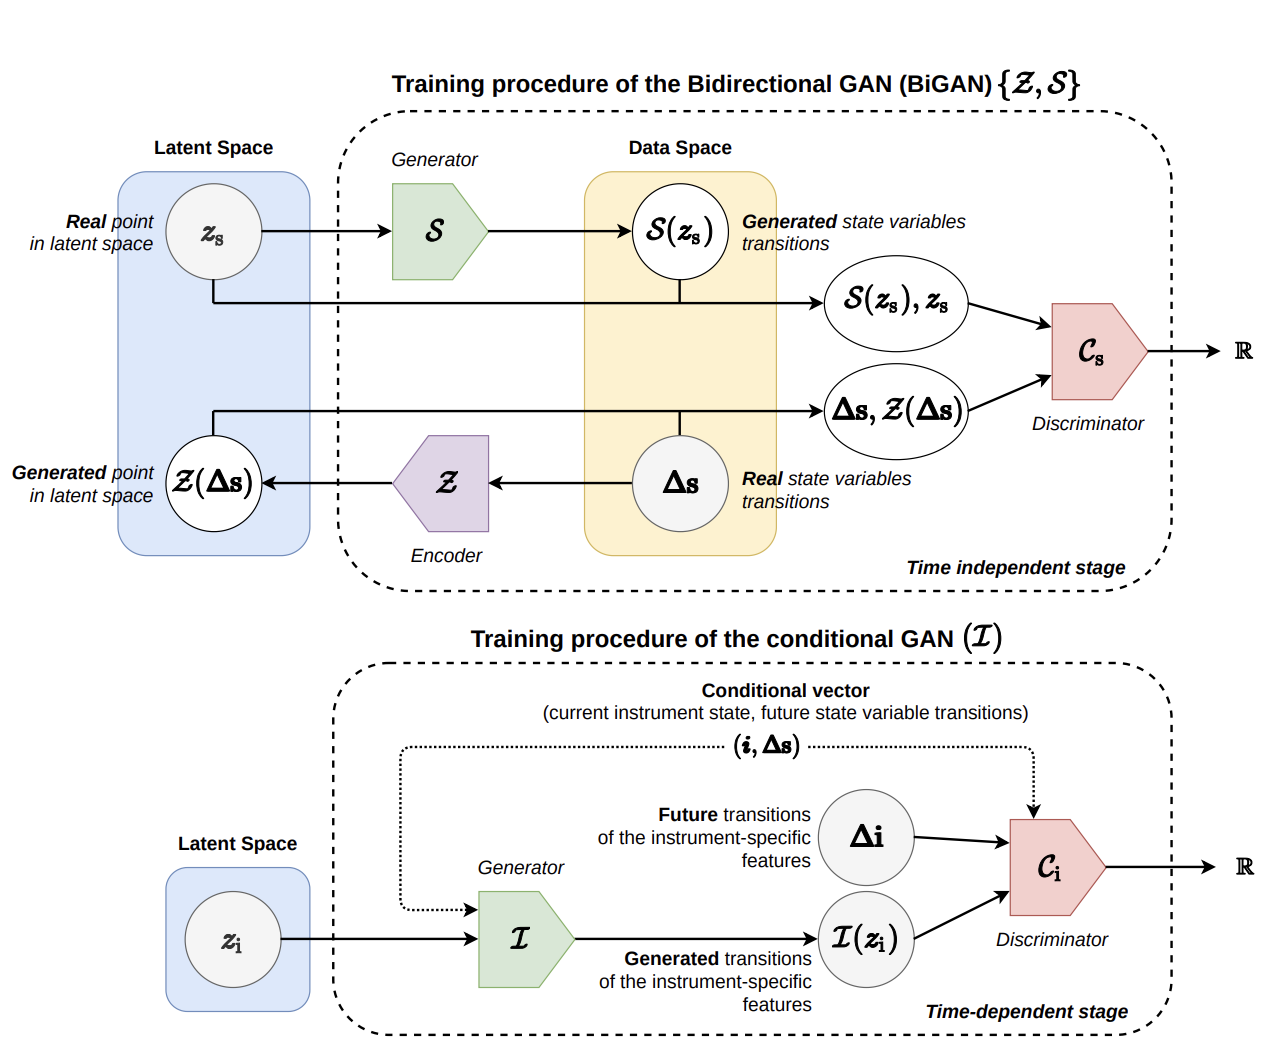
\includegraphics[width=\columnwidth]{bigan_vs_cgan.png}
    \caption{Visual comparison of BiGAN and Conditional GAN training architectures. Adapted from \textcite{rizzato2023generativeadversarial}.}
    \label{fig:bigan-vs-cgan}
\end{figure}

The BiGAN maps latent space to the data space with an autoencoder, similar to the first two components of the TimeGAN. The synthetic time series generated by the trained BiGAN are used as the input for the cGAN, which learns to map each datapoint \textit{y} to a probability score \textit{p} drawn from the dataset distribution of \textit{P} \cite{rizzato2023generativeadversarial}. The cGAN refines the results of the BiGAN by more accurately mapping the data to the probability distribution expected of the data. They perform statistical analysis of their synthetic data generated under four different market conditions (bull market, bear market, volatile market, and debt crisis). They evaluated the synthetic change in stock price from start to end of the time series with the real percent change in stock price \cite{rizzato2023generativeadversarial}. They found similar values for synthetic vs real data, typically with a difference between [-1,2]\%, indicating that their synthetic data was sufficiently accurate to the real data.

\subsubsection{Key Takeaway}
This project demonstrates how synthetic data is a viable way of simulating market scenarios under different macroeconomic conditions. Specific to my project, \textcite{rizzato2023generativeadversarial} found the use of GAN models to be effective for generating synthetic time-series, and were able to compare that synthetic data to real data with a satisfactory degree of accuracy. Their results validate the importance of macroeconomic indicators in financial modelling.

\subsection{Sustainable Economies: Using a Macroeconomic Model to Predict How the Default Rate is Affected Under Economic Stress Scenarios}
\textcite{baltazar2020sustainableeconomies} build a macroeconomic stress-testing framework to predict loan default rates under hypothetical, simulated macroeconomic conditions–a framework they argue would allow banks and policy makers to improve their decision making in economic downturns \textcite{baltazar2020sustainableeconomies}. They use a predefined macroeconomic model rather than machine learning, having that model generate random Monte Carlo simulations \textcite{baltazar2020sustainableeconomies}.\\
Since this is not a machine learning project, my takeaways were not technical but theoretical. They validate the importance of GDP and CPI as revealing macroeconomic indicators, and acknowledge the problem of small datasets for macroeconomic forecasting \textcite{baltazar2020sustainableeconomies}. This study confirmed the relevance and importance of everything I am working on for my project: the use of macroeconomic indicators for understanding economic conditions, the downstream effects of macroeconomic conditions on all aspects of finance and the economy, and the necessity and potential applications of synthetic macroeconomic data in augmenting existing datasets.

\subsection{A Multi-Faceted Evaluation Framework for Assessing Synthetic Data}
This study, by \textcite{yuan2024multifacetedevaluation}, proposes a novel method for the evaluation of synthetic datasets, which they call SynEval. Their evaluation method has three dimensions–fidelity, utility and privacy–of which I am interested in ‘utility’, their measure of the applicability of the synthetic data \cite{yuan2024multifacetedevaluation}.

\subsubsection{Technical Approach}
\textcite{yuan2024multifacetedevaluation} refer to the ‘utility’ of a synthetic dataset as its ability to be used downstream for machine learning. This aspect is what I am most concerned with, as my goal is to create synthetic data that is academically and empirically useful. Downstream machine learning refers to the application of the generated data to training/testing machine learning models. The utility evaluation they proposed is based on a framework referred to as TSTR (Train-Synthetic-Test-Real) \cite{yuan2024multifacetedevaluation}. They perform a study on synthetic data generated by popular LLMs ChatGPT 3.5, Claude 3 Opus, and Llama 2 13B. In this case, they used 50 samples from a software product review dataset to train LLM’s to generate synthetic review-rating data \cite{yuan2024multifacetedevaluation}. They then trained four sentiment classification models; one on the real dataset, and the other three on the synthetic datasets produced by the LLMs \cite{yuan2024multifacetedevaluation}. The sentiment classification models were evaluated on unseen test data, with Mean Absolute Error (MAE) and percentage accuracy of correct classifications used to evaluate the performance of each model. 

\subsubsection{Key Takeaway}
In evaluating the synthetic datasets on downstream machine learning performance, they found that the model trained on synthetic data generated by Claude had a MAE of 1.2929 and accuracy of 67.68\%, which was very comparable to the model trained on real data (MAE 1.3019, accuracy 67.92\%) \cite{yuan2024multifacetedevaluation}.\textcite{yuan2024multifacetedevaluation} results prove that synthetic data can be effectively used on downstream machine learning tasks. Their methodology of using downstream machine learning as an evaluation metric for the quality of synthetic data validates my plan of using a forecasting model trained on synthetic versus real data as an evaluation metric. 

Overall, these studies and prior works demonstrate the viability of GAN models for generating synthetic economic/financial data, the relevance of macroeconomic indicators in research and prediction, and the viability of my proposed evaluation strategies for real versus synthetic data.

\section{3-Week Project}

\subsection{Goal}
The goal of my three-week mini-project was to conduct a test on the downstream evaluation methods that I will be using for the larger project, while at the same time doing a simplified version of the data gathering and processing procedure. The final project aims to generate synthetic datasets using a TimeGAN model, and evaluate the usability of those datasets  with downstream machine learning use. My initial study focused on assessing whether data that is augmented from real data (in this case by adding Gaussian noise) impacts downstream model performance. I also wanted to test whether using a downstream model will be a reasonable evaluation metric for the realism of synthetic data.

\subsection{Data Collection and Cleaning}
I wanted to test my proposed evaluation methods, and get an idea of what the data collection and cleaning process would be like for this project where I combine different countries' datasets. During the data collection process I wanted to test sources for macroeconomic data. In this case I used Federal Reserve Economic Data (FRED) for US GDP and CPI data, and the Office of National Statistics (ONS) for data on the UK, which both had open access, quality data that was easy to retrieve either via API keys or CSV download. During this process I ran into minimal issues with finding data, which is promising for my future project where I intend to use many more countries for input data. However, the formatting was slightly different between countries, and the UK showed a preference for annualized rate of CPI change, so I know now that during the larger data collection I will have to verify that each country publishes data with the same measure of CPI or GDP.\\
When using the actual TimeGAN, it will be trained on each country's data as an independent sequence. For the simple RandomForestRegressor I used in the mini-project, using multiple sequences in training was not an option. However, since my goal was not macroeconomic accuracy, but rather a test of the evaluation procedure and metrics, I decided to just vertically concatenate the data from the two countries into one larger dataset. Using built in tools with Pandas dataframes, it was very easy to normalize GDP and CPI to quarter over quarter percent change.

\subsection{Model Selection and Training}
The RandomForestRegressor (RFR) model requires minimal preprocessing and provides consistent results with a fixed randomized seed. It makes predictions by building a collection of trees like a flowchart using the previous eight data points being used to inform the decision tree process for the next point. Each tree makes its own prediction for the next GDP value, and then the average of all predictions is output. This approach reduces how susceptible to noise the model is, which is important with a smaller dataset. The decision trees naturally don’t rely too heavily on any one feature of the data. A RFR was simple and accurate enough to be used as an example for downstream data use, yet in my real project I will use a more elegant model.

Two RFR were trained, one with the base dataset of real macroeconomic data, and the other noisy dataset augmented with Gaussian noise. Each dataset was first transformed into a supervised learning format, where features consisted of the previous eight quarters (8 lags) of GDP and CPI, and the given target was the GDP change in the next quarter. The datasets were split into 80\% training (224 data points) and 20\% test (56 data points). Both models were tested on the same held-out data from the real dataset, and evaluated on their performance using Mean Squared Error (MSE), Mean Absolute Error (MAE), and coefficient of determination $R^2$ value. 

\subsection{Results}

The results of the model predictions can be seen in \textbf{Figure 2}. Though it is very hard to distinguish between the base and noisy predictions due to very small differences, both can be seen to be pretty good at predicting the general direction of GDP movement, even if they failed to capture the movement at the more volatile moments. Keep in mind that the data splicing makes this an inaccurate representation of GDP changes in the real world, yet the principal is to examine the evaluation metrics and procedure. 

\begin{figure}[h]
    \centering
    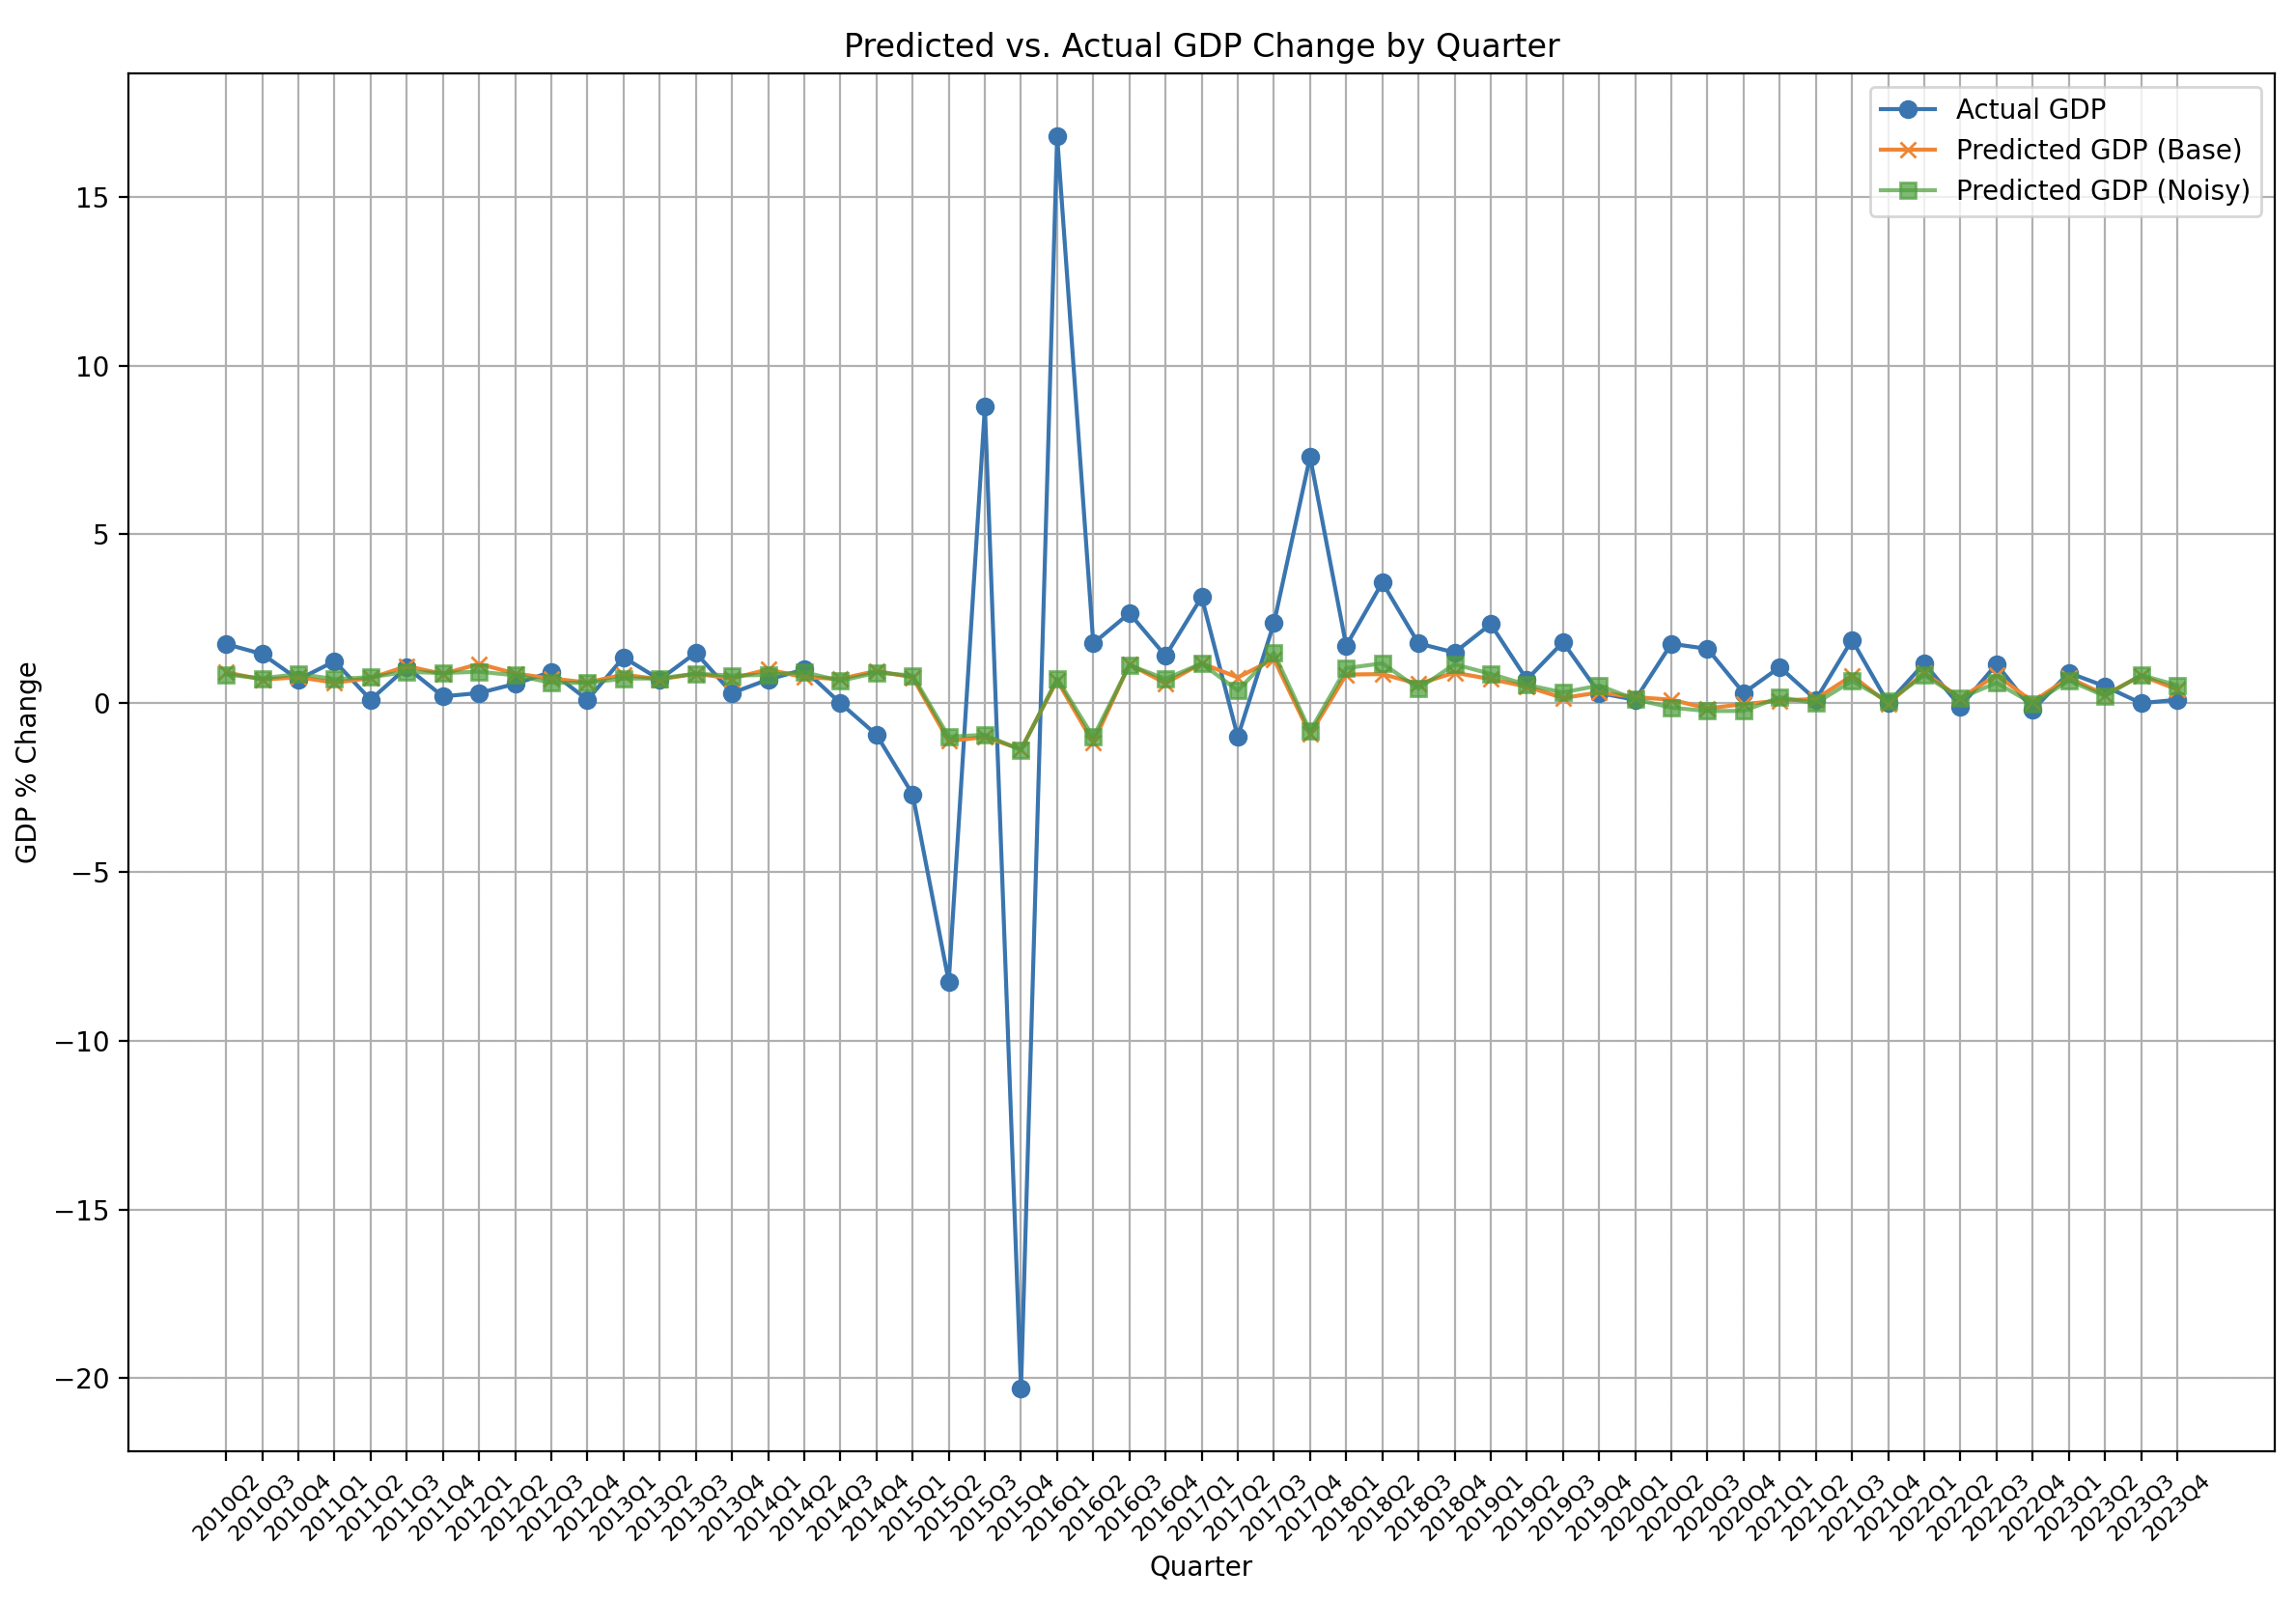
\includegraphics[width=\columnwidth]{pred_vs_actual_gdp.png}
    \caption{RandomForestRegressor Model Predictions on Real and Noise-Augmented Data}
    \label{fig:pred_vs_actual_gdp}
\end{figure}

Though almost negligible, the model trained on noisy data performed slightly better than the base model, although both performed very similarly (see \textbf{Table 1}. $R^2$ values were very low in each case, between 0.05 and 0.06. This implies that the models performed between 5-6\% better than just taking the mean of values. This is to be expected due to the small dataset, limited features, and small absolute values that are very noise-sensitive. The MAE of the noisy dataset was 0.0177 lower than that of the base data, which means that the average absolute error of the model was slightly lower. With a higher $R^2$ value, as well as lower MSE, according to these metrics the noisy model was actually a slightly better predictor of actual GDP values than the base model.\\

\begin{table}[h]
\centering
\caption{Model Performance on Base vs. Noisy Datasets}
\begin{tabular}{|l|c|c|c|}
\hline
\textbf{Dataset} & \textbf{MSE} & \textbf{MAE} & \textbf{R\textsuperscript{2} Score} \\
\hline
Base  & 16.3236 & 1.8422 & 0.0512 \\
Noisy & 16.2091 & 1.8245 & 0.0590 \\
\hline
\end{tabular}
\end{table}

This 3 week project does not prove my goal of showing that synthetically generated data can be used equally effectively on downstream machine learning tasks. However, it does demonstrate that data collection on macroeconomic indicators, processing into uniform format, creation of an augmented dataset, and downstream model comparison are all valid steps for my larger comps project.

\section{Proposed Methods and Fall Timeline}

\subsection{Data Collection}
I am going to train a model to generate synthetic quarterly macroeconomic indicators (eg. GDP and inflation rate) using input datasets drawn from multiple countries. In order to maintain some consistency in the input data, as well as consistency in the type of economies it is generating data for, I will be training the model using input data only from developed countries with relatively free market economies. This excludes markets like China, where capital controls limit the inflation rate and exchange rates to other countries, and may have repressive or inflationary effects on GDP.\\
\indent{}I will retrieve my data for the US from the Federal Reserve Economic Data (FRED), and for other countries will use the Organization for Economic Cooperation and Development (OECD), International Monetary Fund (IMF), and the World Bank. All of these sources have accurate, public data available for macroeconomic indicators. As for my chosen indicators, as described in the technical background section I will be using CPI, unemployment rate, and GDP, and ideally interest rate and real wage if I can find consistent data across countries. I will focus on countries with reliable quarterly GDP and CPI data, quarterly (or similar) reporting data, and minimal gaps in coverage. \\ 
\indent{} Overall this approach will build on the process tested during my three-week project, where I gathered GDP and CPI data from the US and UK. Any minor differences in reporting formats (like annualized CPI for the UK in the three-week project) will be accounted for country by country.\\
\indent{}The preprocessing for these datasets should be fairly simple. In the case of missing data those rows will have to be dropped from the dataset. Each country's data will be treated as an independent time series where each row represents one quarterly time step. For the datasets to be consistent, GDP and CPI will be normalized to quarter over quarter percent change, which will get rid of the issue of absolute values differing between countries. Unemployment rates are far more comparable across countries, so they don’t need to be normalized. While each country’s data will be processed into the same structure and labeling, they will be fed into the TimeGAN as a 3D dataset with shape $[N, T, F]$, described in \textbf{section 2.2.2}. One of the strengths of the TimeGAN model is that it takes numerous input sequences to train from to learn the temporal aspect of how data-points are related. 


\subsection{Model Training}
The model will be adapted from the open-source TimeGAN implementation available at \href{https://github.com/jsyoon0823/TimeGAN/tree/master/}{GitHub} \cite{yoon2019timeseriesgenerative}. The objective is to train a TimeGAN model to generate realistic macroeconomic time series using the multi-country, normalized dataset. By training the TimeGAN on a number of different countries, the model will learn macroeconomic relationships across different contexts without compromising the underlying relationships (eg. the relationship between GDP and CPI is the same across countries). This is the reason why macroeconomic indicators are uniquely suited for such a project, as their relationships don’t vary by country. The diversity of countries sampled will improve generalizability and reduce overfitting to US specific data, which is especially important given the fact that only four data points are taken annually for each country.\\
\indent{}Once the model has learned to generate latent sequences to mimic the structure of the input data, I will pass random noise from a standard distribution through the generator portion of the TimeGAN \cite{yoon2019timeseriesgenerative}. The generator will then map this noise to a sequence of time series points in the latent space, which will then be decoded using the recovery network portion of the TimeGAN \cite{yoon2019timeseriesgenerative}. The result will be time series sequences of data of the same length, dimensionality and structure as the training data.


\subsection{Results Evaluation}
To perform the statistical analysis of the synthetic data, I will use the data tests designed specifically for evaluation of generated data that I discuss in the technical background and prior work sections. Namely this will be a Wasserstein-Cramer's V test, novelty test, and anomaly detection test. These tests will be performed on the synthetic data output from the TimeGAN as a direct comparison to the real data.\\
\indent{} As in the mini-project, the core prediction task will be to forecast-next quarter GDP using the previous quarters of GDP, CPI, ect. The key different in the fall is that one model will be trained on real data and the other on fully synthetic TimeGAN-generated data. They will be tested on the same held-out test set, and my comparison will use the same metrics as in the mini-project: MAE and $R^2$.


\subsection{Weekly Timeline}
\begin{table}[h]
\small
\caption{Proposed Week-by-Week Project Timeline}
\begin{tabular}{|p{1.2cm}|p{6.1cm}|}
\hline
\textbf{Week} & \textbf{Goal} \\ \hline
1--2  & Data collection and cleaning. \\
\hline
3--4  & mini-TimeGAN training, debugging, and tuning. \\
\hline
5--6  & Full TimeGAN training on complete dataset. \\
\hline
7--8  & Statistical evaluation of synthetic output. \\
\hline
9--10 & Forecasting model experiments. \\
\hline
11    & Compare results of synthetic and real data. \\
\hline
12    & Begin write-up and drafting the paper. \\
\hline
13    & Finalize paper and visualizations of results. \\
\hline
14    & Prepare presentation and submit final project. \\
\hline
\end{tabular}
\arrayrulecolor{black} % reset rule color
\end{table}


\section{Metrics and Result Thresholds}
To evaluate whether my synthetic dataset is comparable to real data and has real-world utility, I plan to use a mix of the statistical methods outlined by \textcite{livieris2024anevaluationframework}, along with a downstream machine learning comparison similar to \textcite{yuan2024multifacetedevaluation}.

For the statistical comparison between the real and synthetic datasets, I will use the Wasserstein-Cramer’s V test, Novelty test, and Anomaly detection test as used by \textcite{livieris2024anevaluationframework}. The Wasserstein-Cramer’s V test will give me a picture of the similarity of the distribution of the synthetic data to real. For Wasserstein-Cramer’s V test, I will be aiming for a value of 5, with lower values being better. \textcite{livieris2024anevaluationframework} achieved a Wasserstein-Cramer’s V test value of 11.0 at the lowest, yet they used fewer data points than I hope to use and trained a simpler model. The novelty test will evaluate the presence of new instances inside the dataset. I will aim for a mean novelty score between [0.2,0.5]. Anything too close to 0 indicates that the data may be overfit and doesn’t introduce any new data points, yet anything higher than 0.5 may be too far from the real distribution. For the anomaly rate, I hope to achieve a value of  5\%, which represents the portion of data points identified as anomalies.

In terms of downstream machine learning evaluation, I plan to compare the performance of two forecasting models, one trained on synthetic and one trained on real data. The goal of each model will be to predict the rate of GDP change over time using unseen test data. To compare the models, I will use Mean Absolute Error and percent accuracy, as done by \textcite{yuan2024multifacetedevaluation} in their evaluation of the utility of synthetic data. Since GDP will be expressed in percentage change with the majority of values being less than 5\%, I will aim for a MAE of below 0.5 on my synthetic data, but as long as it has an MAE within ±0.05 of the real data then I will find that to be an acceptable result. As for accuracy, the synthetic data model should fall within ±2\% accuracy of the real data model. If both of these requirements are met then I can determine that my synthetic data is able to be effectively used on downstream machine learning tasks.

\section{Ethical Considerations}
Though the overall goal of my project is to generate realistic and usable synthetic macroeconomic time-series, it is important also to assess the ethical implications of such a project. The primary ethical concern with such a project is the question of who actually benefits from improved economic simulation, and who may be unintentionally excluded from those benefits.
\textcite{ravallion2021macroeconomicmisery} point out how changes in macroeconomic conditions have disproportionately negative impacts on the poorest Americans. Unemployment rate or inflation rates for example, may negatively impact the value of the wealth of upper class Americans, but won’t have any impacts on their daily lives \textcite{ravallion2021macroeconomicmisery}. The poor however, are placed under immense burden from macroeconomic changes.\\
\indent{}The major concern is that improved macroeconomic modelling only serves to benefit those with the financial literacy and wealth to take advantage of it–particularly banks, policymakers, and wealth investors. As such, macroeconomic modelling is likely to be used to benefit these upper-class groups, rather than improve the financial standing and financial literacy of the lower class.
\indent{}There is also the risk that synthetic data is used by a powerful actor (eg. the Federal Reserve System in deciding interest rates) without disclosure of where that data came from or why it was used. Since macroeconomic factors are impactful to all, anybody who is in a policy making position must be transparent and accountable for the data they use. Since the general public, and even data-scientists may not know exactly what patterns an algorithm is learning in training, there is the potential that synthetic data abstracts real world conditions, creating incomplete or untrustworthy datasets that are then used in vital decision making. \\
\indent{}On the topic of ethics in computer science, the discussion of algorithmic decision making in credit-scoring and loan rating has been controversial, as it obscures the process behind making very impactful decisions on people's lives. The use of synthetic macroeconomic data in decision making poses the same risks.
\indent{}Though the aim of this project is academic research into synthetic data and macroeconomic indicators, advancements in macroeconomic modelling techniques risk further exacerbating the divide between those who have the knowledge and wealth to take advantage of financial information and those who don’t. Transparency on the generation process of synthetic data is vital to mitigating these risks.


\printbibliography

\clearpage

\onecolumn

\end{document}
